\documentclass[12pt]{article}
\usepackage{amsfonts,amsmath,amsxtra,amsthm}
\usepackage{amssymb}
\usepackage[utf8]{inputenc}
\usepackage{xcolor}
\usepackage{tikz, subfig, pgfplots, ifthen}
\usepackage{tcolorbox}

\begin{document}

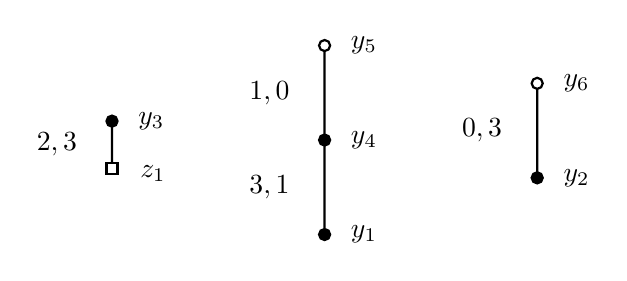
\begin{tikzpicture}
	\def\l{1.2};
	\def\r{2};
	\def\s{2.7}
	\draw[thick, fill] (-\s,-0.8*\l)  circle (\r pt) node[xshift = 0.5cm] {$y_{3}$} -- node[xshift = -0.7cm] {$2, 3$} (-\s, -0.8*\l-0.5*\l);
	\draw[thick, fill = white] (-\s cm -\r pt, -0.8*\l cm -0.5*\l cm - \r pt ) rectangle (-\s cm + \r pt, -0.8*\l cm -0.5*\l cm + \r pt)  node[xshift = 0.45cm, yshift = - 2*\r pt]{$z_{1}$};
	\draw[thick, fill] (0,0) -- node[xshift = -0.7cm] {$1, 0$} (0,-\l) circle (\r pt) node[xshift = 0.5cm] {$y_{4}$} -- node[xshift = -0.7cm] {$3,1$} (0,-2*\l) circle (\r pt) node[xshift = 0.5cm] {$y_{1}$} ;
	\draw[thick, fill = white] (0,0) circle (\r pt) node[xshift = 0.5cm] {$y_{5}$};
	\draw[thick, fill] (\s,-0.4*\l) -- node[xshift = -0.7cm] {$0, 3$} (\s,-0.4*\l-\l) circle (\r pt) node[xshift = 0.5cm] {$y_{2}$} ;
	\draw[thick, fill = white] (\s,-0.4*\l) circle (\r pt) node[xshift = 0.5cm] {$y_{6}$};
	\end{tikzpicture}

\end{document}